\section{Explanation}

Here we present some result on logistic regression. We diagnose the weights to see the contribution of each attributes. Here are our visualization results.

\begin{figure}[ht]
    \centering
    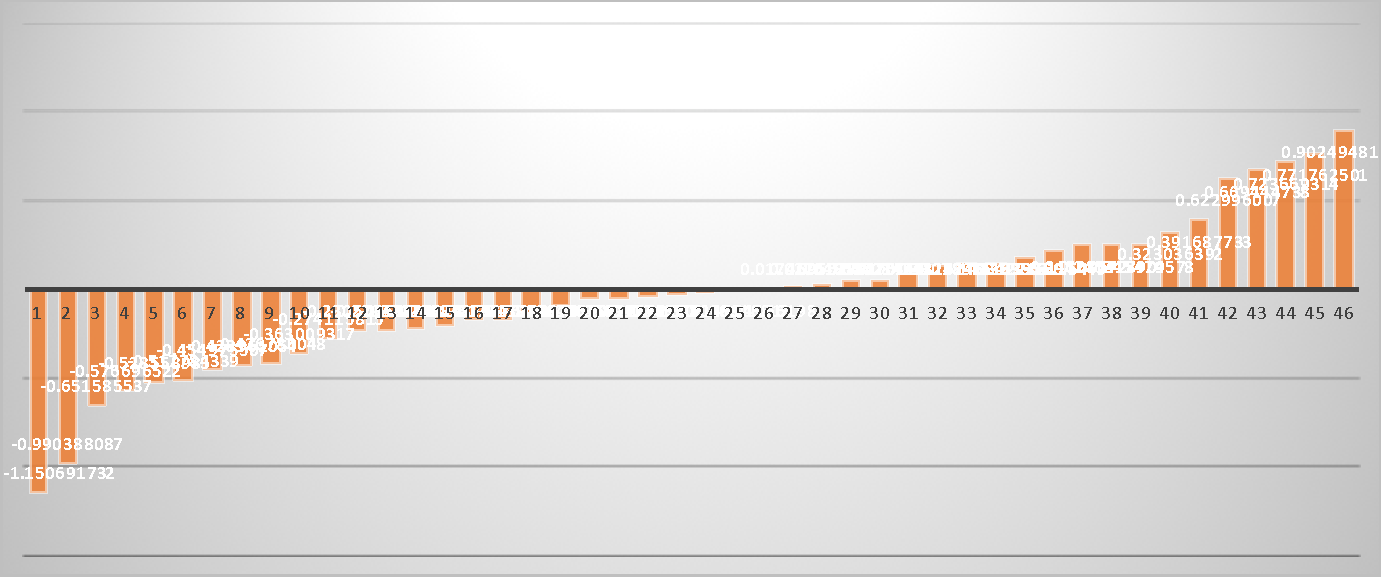
\includegraphics[width=1\linewidth]{img/ttt.pdf}
    \caption{weight in logistic regression.}
\end{figure}

We can see the right most attributes, which are 'profession', `contact', 'schooling',  and the left most atributes are `loan', 'housing'. We can that the right most attributes can provide more positive contributions, which denote that if the custom have good profession, and high contact fraquency, we have more chance to market. And the left most attributes denote they provide bad effect to final market results. If someone have high loan and housing load, we have little chance to market.

